\chapter{Árboles de Búsqueda Equilibrados}
La inserción como la eliminación de elementos de un ABB determinan su grado de equilibrio, por ende la suceción inserción o eliminación de elementos del mismo puede alterar el equilibrio del árbol.

Sabemos que el coste de las operaciones \texttt{buscar()}, \texttt{insertar()} y \texttt{eliminar()} depende de la altura del árbol (el caso más desfavorable vimos que era \(O(n)\) `lista').

Este equilibrio nos permite garantizar un coste proporcional a la mínima altura posible del árbol, consiguiendo un coste mínimo de \(O(log_{2}\ n)\), por tanto, es muy importante que a la hora de insertar o eliminar elementos mantengamos el árbol lo más equilibrado posible.

Encontramos dos tipos de árboles equilibrados los \textbf{árboles AVL} y los \textbf{árboles ARN}.

\section{Árboles AVL}
Un \textbf{árbol AVL} es un tipo de ABB equilibrado, la resta de la altura del subárbol derecho menos la altura del subárbol izquierdo del mismo nodo se denomina \textbf{factor de equilibrio de nodo} (esto garantiza el coste logarítmico).

Decimos que un árbol está equilibrado cuando su factor de equilibrio es -1, 0 ó 1 en todos sus nodos.

Como hemos comentado previamente, la inserción y la eliminación de elementos pueden verificar la condición de equilibrio del árbol y si es necesario, reequilibrarlo mediante la rotación de nodos (intercambios).

En el peor caso, el tiempo de inserción, eliminación y búsqueda están en coste \(O(log\ n)\).
\subsection*{Diferencia entre AVL y No AVL}
\begin{figure}[h]
  \begin{minipage}{.5\textwidth}
    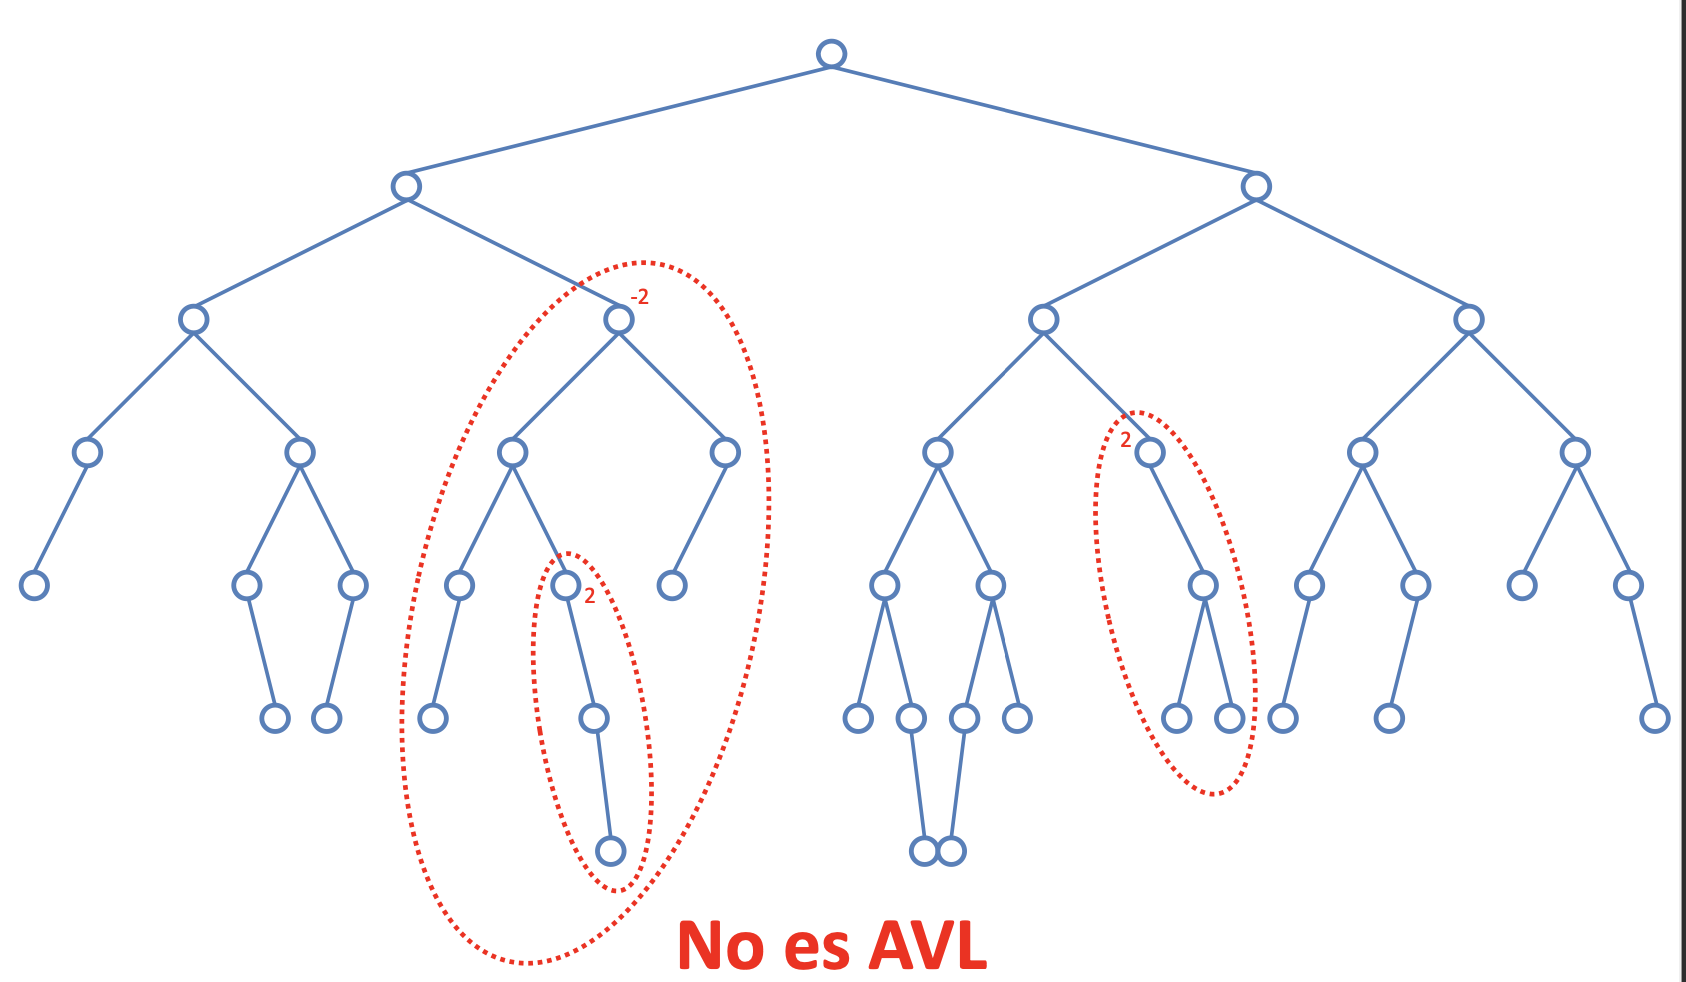
\includegraphics[width=\textwidth]{assets/avl1.png}
  \end{minipage}
  \hfill
  \begin{minipage}{.5\textwidth}
    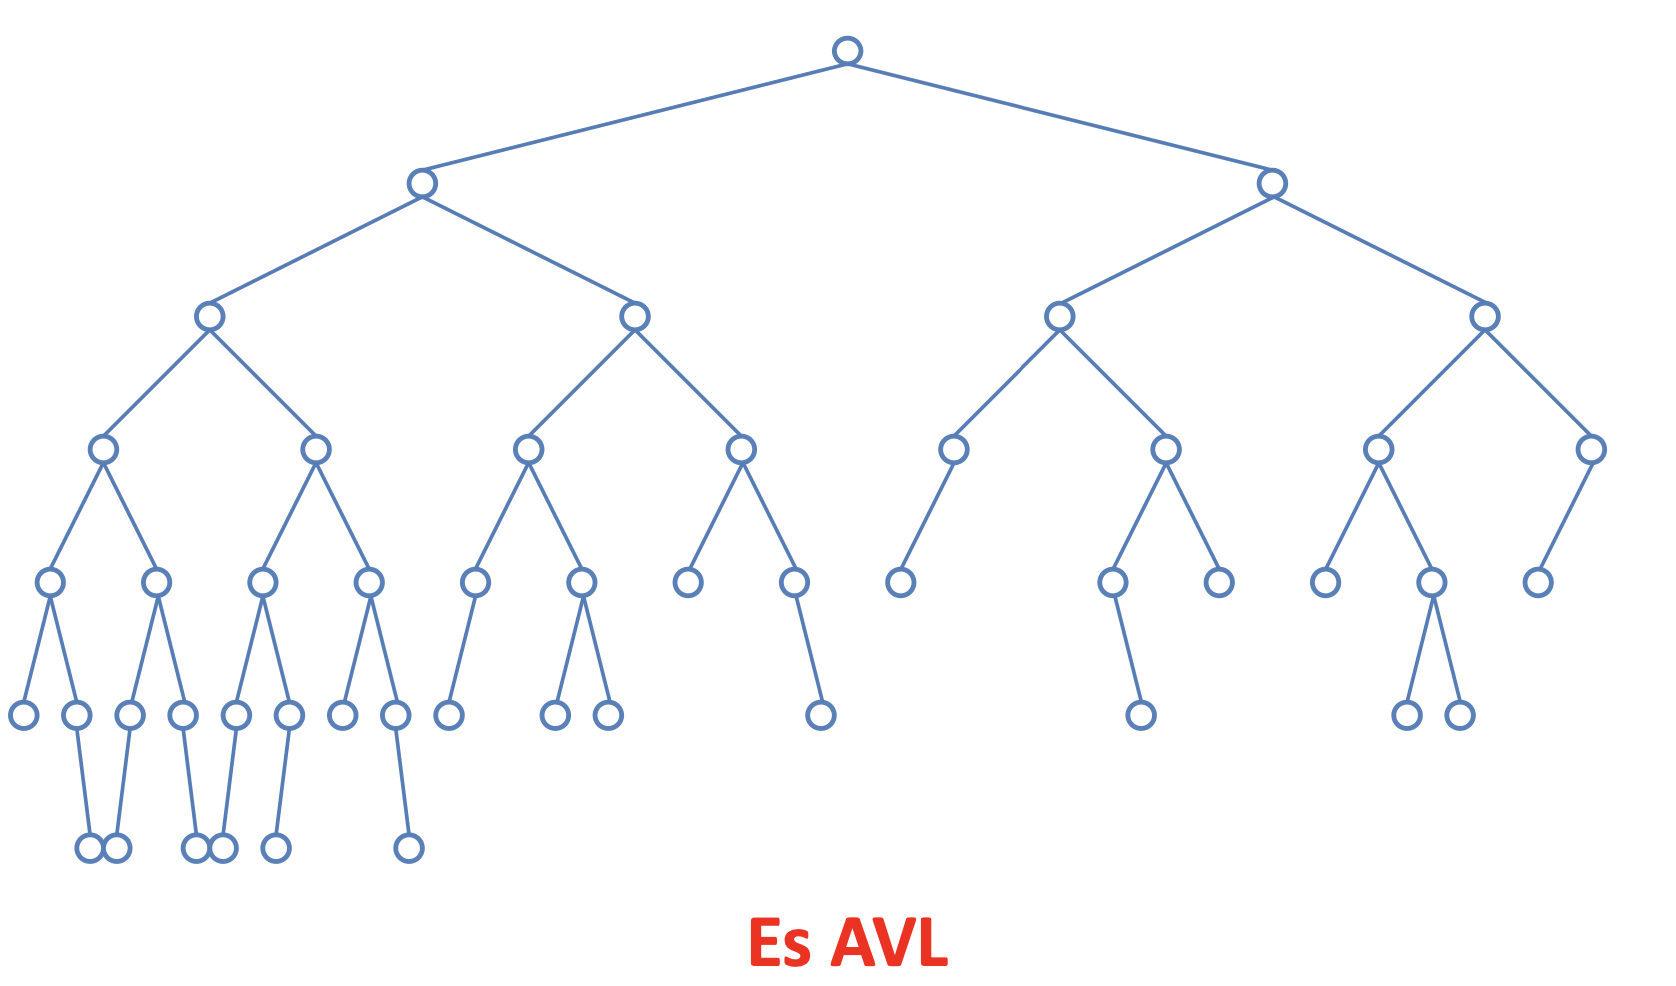
\includegraphics[width=\textwidth]{assets/avl2.png}
  \end{minipage}
  \caption{Diferencia entre No AVL y AVL}
\end{figure}
\newpage
\section{Árboles ARN}
Un \textbf{árbol ARN} ó \textbf{árbol rojinegro} es un ABB que representa un \textit{árbol B} de orden 3 (árbol 2-3), el cual está equilibrado (tiene todas las hojas en el mismo nivel).
\begin{figure}[h]
  \begin{minipage}{.4\textwidth}
    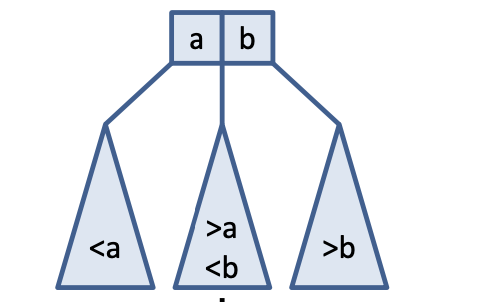
\includegraphics[width=\textwidth]{assets/arn1.png}
  \end{minipage}
  \hfill
  \begin{minipage}{.6\textwidth}
  Si tenemos \(k\) claves, entonces tenemos \(k+1\)caminos, por tanto, si tenemos un árbol 2-3, tendremos 2 clave y 3 caminos.\\
  Si tenemos 2 claves el desequilibrio va a ser 1.\\
  Siempre va a existir un nodo negro (valor más grande del par) pero puede existir o no un nodo rojo (valor más pequeño del par).
  \end{minipage}
\end{figure}

Esta representación permite una implementación más sencilla de inserciones y eliminaciones, ya que solamente comparamos los valores de cada nodo y no tenemos que hacer uso de estructuras complejas como los punteros.

Todo nodo \textbf{raíz} se denomina nodo negro, mientras que todo \textbf{hijo izquierdo} de esa raíz se denomina nodo rojo. Otra cosa a tener en cuenta es que todos los hijos de un nodo \textbf{rojo} son nodos \textbf{negros}, véase en la (\textit{Figura 5.2: Ejemplo de árbol rojinegro}).
\begin{figure}[h]
  \begin{center}
    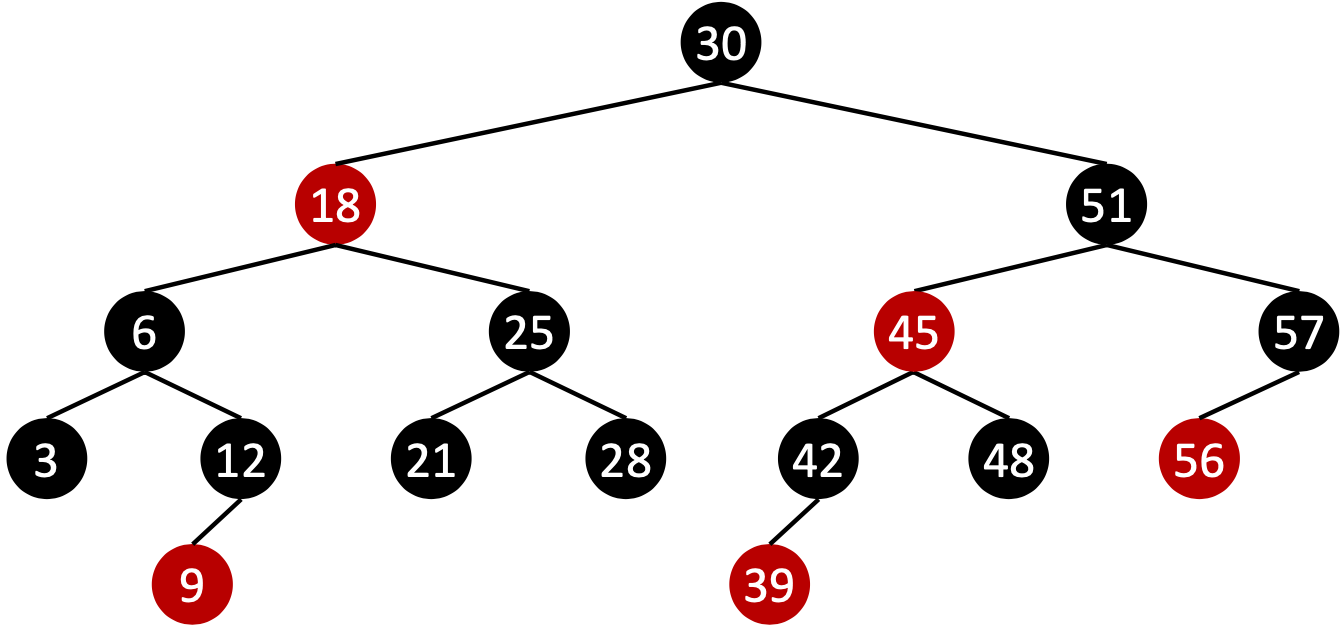
\includegraphics[width=0.7\textwidth]{assets/arn2.png}
  \end{center}
  \caption{Ejemplo de árbol rojinegro}
\end{figure}

\subsection*{Inserción y Eliminación}
Se realizan igual que en un ABB (Árbol Binario de Búsqueda) pero deben de representar correctamente el árbol 2-3 subyacente, es decir, tenemos que realizar cambios de color y rotaciones (operaciones internas) en los nodos.
\subsection*{Operaciones internas}
Encontramos las operaciones de rotaciones y repintado las cuales tendremos que usar a la hora de insertar y eliminar nodos:
\begin{itemize}
  \item \textbf{Rotación →} Recolocan los nodos del árbol conservando la propiedad de orden/búsqueda.
  \item \textbf{Repintado →} Cambia de color a los nodos.
\end{itemize}

La efiencia en los árboles rojinegro dependen de la altura del mismo, es decir, para un árbol rojinegro con \(n\) nodos tiene una \textbf{altura} \(h \leq 2log_{2}\ n\) y dado que las operaciones de \textbf{inserción}, \textbf{búsqueda} y \textbf{eliminación} tienen un peor tiempo de ejecución proporcional a la altura del árbol, entonces estás operaciones tienen un coste de \(O (log\ n)\).

\section{AVL vs ARN}
Los árboles AVL están \textit{más equilibrados} que los árboles ARN, ya que el desequilibrio máximo de los AVL es 1, además que en los AVL las búsqueda de elemento son \textit{más rápidas}.\\ 
Por otro lado, los árboles ARN son \textit{más flexibles} por lo que las inserciones y eliminaciones de elementos son más rápidas.
\begin{figure}[h]
  \begin{center}
    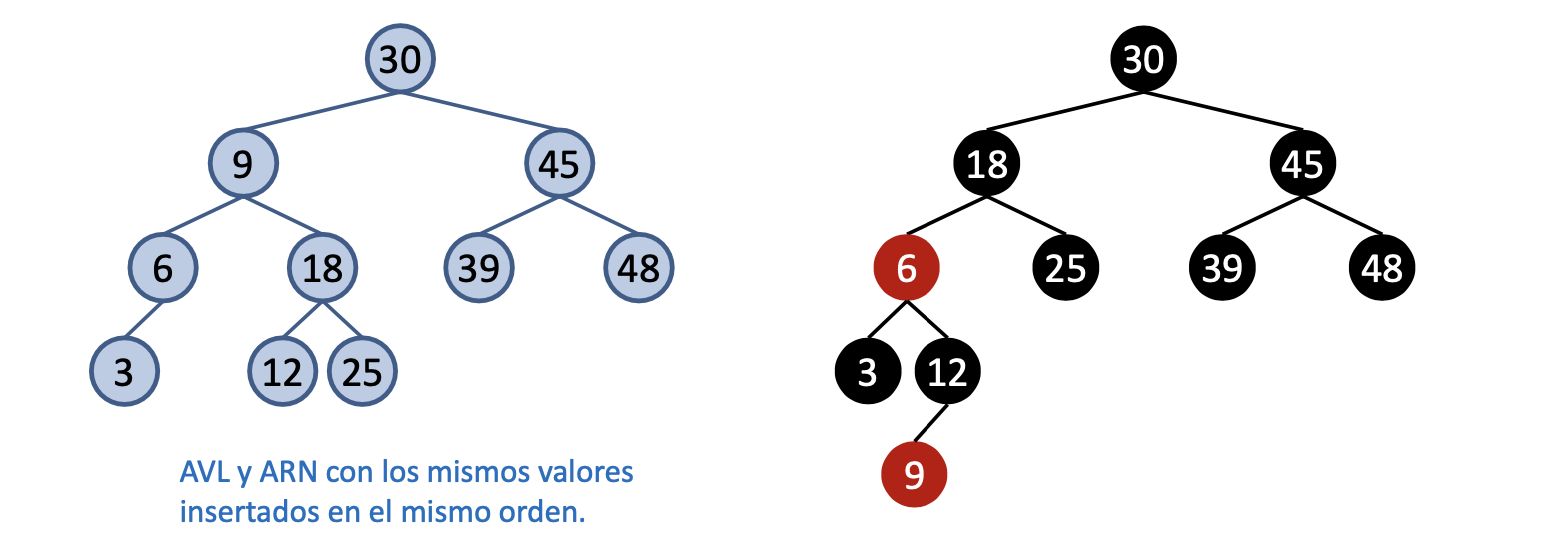
\includegraphics[width=\textwidth]{assets/avl3.png}
  \end{center}
  \caption{Diferencia entre AVL y ARN}
\end{figure}

Sin embargo, estas diferencias comentadas, en la práctica respecto al rendimiento global es inapreciable.
